\documentclass[12pt,a4paper,]{scrreprt}

\usepackage{filecontents}
\usepackage[ngerman]{babel}				% Deutscher Sprachsupport
\usepackage[onehalfspacing]{setspace} 	% Zeilenabstand 1,5
\usepackage[utf8]{inputenc}				% Sonderzeichen 
\usepackage{relsize,booktabs,tikz}

\usepackage{biblatex}
\addbibresource{\jobname.bib}
\usepackage[T1]{fontenc}
\usepackage{lmodern}
\usepackage[
labelfont=sf,
hypcap=false,
format=hang,
width=0.8\columnwidth
]{caption}
\usepackage{graphicx,array,siunitx,multicol,capt-of,amsmath,ulem,amsthm}					% Anderes
\let\phi\varphi
\setkomafont{chapter}{\fontsize{20bp}{22.2bp}\selectfont\bfseries}

\setkomafont{chapter}{\fontsize{14bp}{18.8bp}\selectfont\bfseries}
\setkomafont{section}{\fontsize{12bp}{14.4bp}\selectfont\bfseries}
\usepackage{hyperref}

\renewcommand{\chapterheadstartvskip}{\vspace*{-1\topskip}}
\renewcommand{\chapterheadendvskip}{\vspace*{0.8\topskip}}
\begin{filecontents*}{\jobname.bib}
	@book{ art:test,
  		author = {Wikipedia, Isentropenexponent},
  		title  = {\url{https://de.wikipedia.org/wiki/Isentropenexponent}},
  		publisher = {de.wikipedia.org},
  		year = {abgerufen am 04. Dezember 2016},
}
\end{filecontents*}
%---------------------------------------------------------------------------------------------------------------------------------------------------------------
% Ende der Einstellungen
%---------------------------------------------------------------------------------------------------------------------------------------------------------------

%---------------------------------------------------------------------------------------------------------------------------------------------------------------
%Ab hier gibt es Inhalt
%---------------------------------------------------------------------------------------------------------------------------------------------------------------
\begin{document}

\title{Adiabatenexponent \\ (2. Korrektur)}
\author{Henrik Jäger \\ 3114168 \and Lena Majer \\ 3115808}
\subtitle{W43a \\  Assistent: André Haug}
\subject{Physikalisches Praktikum I}
\publishers{Universität Stuttgart}
\date{Versuchstag: 1. Dezember 2016 \\ Erstabgabe: 8. Dezember 2016 \\ Abgabe der Korrektur: 21. Dezember 2016 \\ Abgabe der Zweitkorrektur: 19. Januar 2017}
%\thanks{Assistent: Sascha Kolatschek}

\maketitle% Titelei

\tableofcontents   %Inhaltsverzeichnis
\pagebreak

\captionsetup{width=0.8\linewidth}

\chapter{Einleitung}
\section{Ziel}
In diesem Versuch soll der Adiabatenexponent von mehreren Stoffen bestimmt werden. Zu bestimmen sind die Adiabatenexponenten von den Gasen Luft (stellvertretend für N$_2$), Kohlenstoffdioxid (CO$_2$) und Argon (Ar).
\section{Grundlagen}
Wenn man mit Gasen zu tun hat, geht man häufig von idealen Gasen aus. Hierbei spielt das ideale Gasgesetz eine wichtige Rolle:\\
\begin{equation}
p\cdot V=n\cdot R\cdot T,
\end{equation}
$p$ entspricht dem Druck , $V$ entspricht dem Volumen, $n$ bezeichnet die Molzahl, $R$ ist die allgemeine Gaskonstante und $T$ entspricht der Temperatur.\\
Bei idealen Gasen gibt es unterschiedliche thermodynamische Prozesse. Unter einem isochoren Prozess versteht man ein Gleichbleiben des Volumens. \\
Unter einer adiabatischen Zustandsänderung versteht man eine Zustandsänderung bei der gilt:
\begin{equation}
P\cdot V^\gamma = konstant
\end{equation}
$\gamma$ kann durch spezifische Kapazitäten berechnet werden. Dabei steht $c_v$ für die Wärmekapazität bei konstanten Volumen und $c_p$ für die Wärmekapazität bei konstanten Druck.\\
\begin{equation}
	\gamma = \frac{c_p}{c_v}
\end{equation}
$\gamma$ kann auch experimentell bestimmt werden. Hierfür nimmt man eine Gasfeder zur Hilfe. Die hierfür nötige Bewegungsgleichung der Gasfeder lautet:\\
\begin{equation}
m \cdot \ddot{x} + \gamma \cdot p_0 \cdot  \frac{A^2}{V_0 } \cdot x=0 
\end{equation}
Diese Differentialgleichung beschreibt einen harmonischen Oszillator. Dessen Lösung, sowie die Formel für die Frequenz sind schon bekannt.
Die Frequenz entspricht:\\
\begin{equation}
f = \frac{1}{2\pi \sqrt{\frac{m}{D}}}= \frac{1}{2 \pi \cdot \sqrt{m \cdot \frac{V_0}{ \gamma \cdot p_0 \cdot A^2}}}
\end{equation}

Wie die Energie sich in thermodynamischen Prozessen verhält, wird im ersten Hauptsatz der Thermodynamik beschrieben: \\
\begin{equation}
dU = dQ  p \cdot dV
\end{equation}
$U$ steht für die innere Energie. Als Thermische Energie wird $Q$ bezeichnet. Es gilt:\\
\begin{equation}
\Delta Q = C \cdot \Delta T 
\end{equation}
$C$ nennt man die Proportionalitätskonstante oder Wärmekapazität. \\
$C$ kann auf zwei verschiedene Methoden bestimmt werden.  Zum einen kann einem Körper eine bestimmte Wärmemenge zugefügt werden und die daraus resultierende Temperaturänderung gemessen werden.\\
Es können aber auch zwei Körper aneinander gelegt werden, um eine gemeinsame Temperatur zu erhalten. Durch diese gemessene Temperatur und die bekannte Wärmekapazität eines Körpers kann die Wärmekapazität des anderen Körpers zu bestimmen.
\pagebreak

\chapter{Messprinzip mit Skizze und Versuchsablauf}
\begin{center}
    		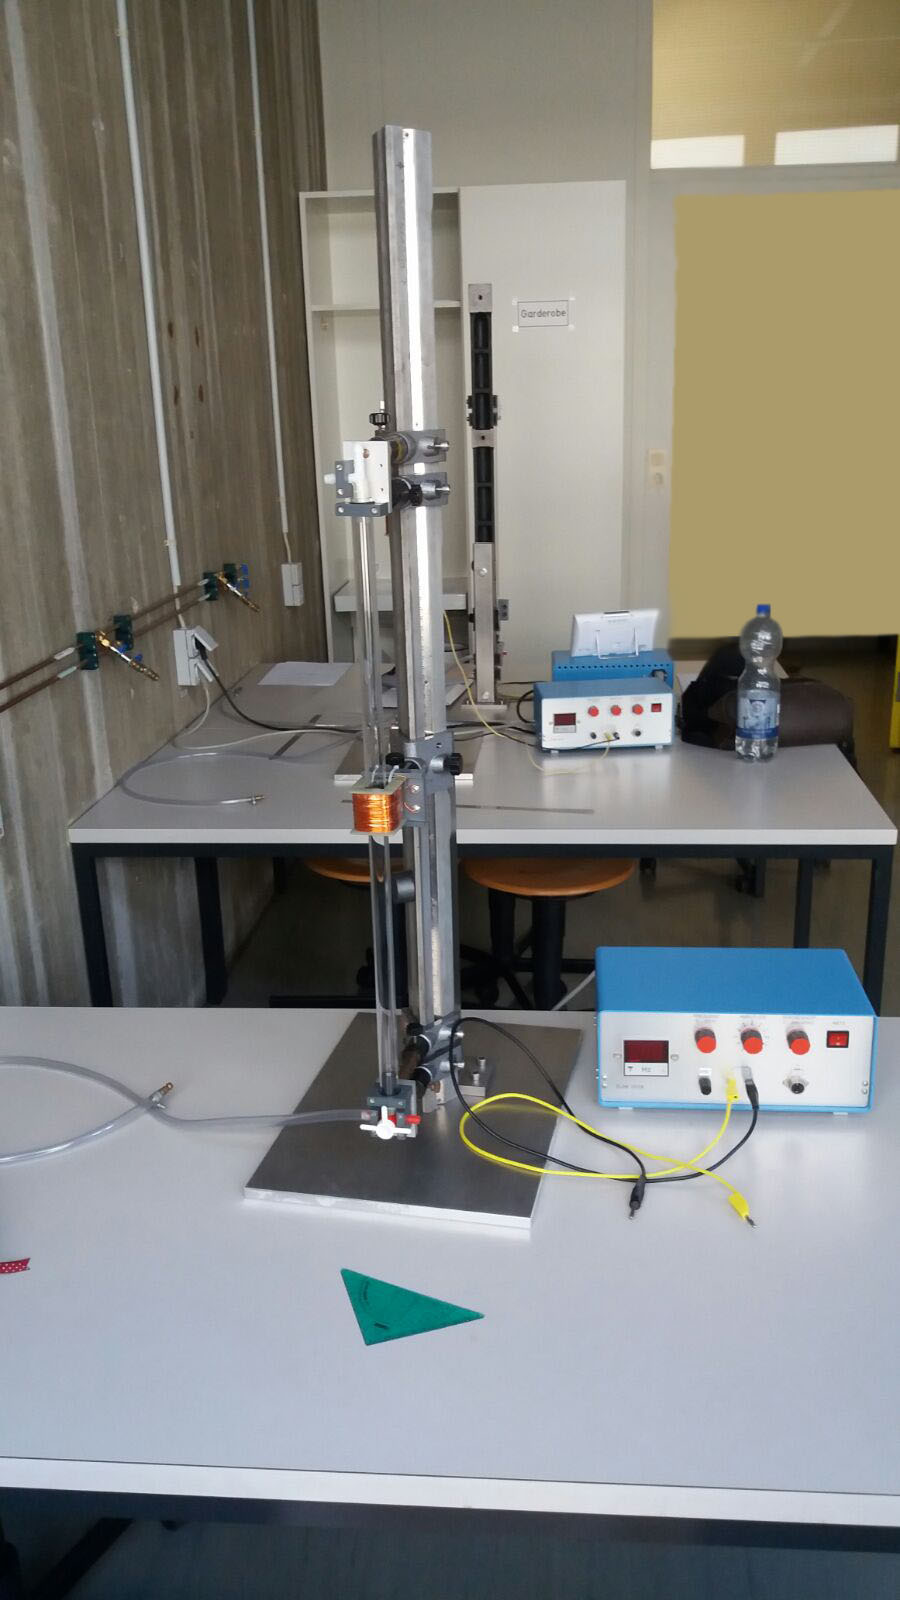
\includegraphics[scale=0.2]{Daten/aufbau.jpeg}
    	\end{center}
    	\captionof{figure}[Seite 1]{Versuchsaufbau bestehend aus einem Glaszylinder und Gaseinlassventil, einem beweglichen Kolben mit Permanentmagneten. Um das Glasrohr sitzt eine Spule  für das magnetische Wechselfeld.}
\ \\
Hierfür wird ein Glaszylinder verwendet. Dieser schließt ein Gasvolumen $V$ ein. In diesem Glaszylinder befindet sich ein Kolben mit Permanentmagnet, der möglichst reibungsfrei gleiten kann. Um den Zylinder befindet sich eine bewegliche Spule. \\
\\
Um den Adiabatenexponenten bestimmen zu können, wird die Resonanzfrequenz in Abhängigkeit des eingeschlossenen Luftvolumens bestimmt. \\
\\
Mit einem außen an den Zylinder gehaltenen Magneten wird der Kolben angehoben. Durch Anlegen eines konstanten Magnetfelds wird der Kolben in einer bestimmten Höhe gehalten. Die Gewichtskraft wird damit kompensiert.\\
\\
Durch Anlegen eines Wechselmagnetfelds wird der Kolben in Schwingung versetzt. Sobald der Kolben in Bewegung ist, wird versucht die Resonanzfrequenz einzustellen. Die Resonanzfrequenz ist erreicht, wenn die Amplitude des schwingenden Kolbens maximal ist.\\
\\
Nachdem die Resonanzfrequenz erreicht ist, wird die Höhe des Kolbens gemessen, um das eineschlossene Volumen bestimmen zu können. \\
\\
Das Vorgehen wird sieben Mal wiederholt.\\
\\
Anschließend werden dieselben Messungen auch für die Gase Argon und CO$_2$ durchgeführt. Auch hier werden jeweils acht verschiedene Volumina untersucht.\\
\\
Bevor die Messungen gestartet werden können, müssen jeweils Zylinder und die Zugangsschläuche mit dem entsprechendem Gas gespült werden.
	\pagebreak
    
\chapter{Formeln}

Zur Berechnung des Adiabatenexponenten wird die Formel aus der Versuchsanweisung$^[$\footnote{Versuchsanleitung W43, Anfängerpraktikum, Universität Stuttgart. Stand: 29.09.2016}$^]$ verwendet:
\begin{align}
     		\gamma = \frac{4\pi^2 m V_0 f_0^2}{A^2 p_0}
            \label{gamma}
      \end{align}
      $m$ steht für die Masse,  $V_0$ für das eingeschlossenen Gasvolumen, $f_0$ entspricht der Resonanzfrequenz des schwingenden Kolbens und $p_0$ steht für den Druck.
	\pagebreak



	\chapter{Messwerte}
    	\begin{center}
    	\begin{tabular}{c|cccccccc}
        	$l ~ [ \text{m}]$ & 0,45 & 0,40  & 0,35 & 0,30 & 0,25 & 0,20 & 0,15 & 0,10 \\ \hline
			$f_0 ~[ \text{Hz}]$& 13,4 & 14,1 & 15,5 & 16,4 & 17,8 & 19,7 & 22,8 & 27,4                
		\end{tabular}
			\captionof{table}[luft]{Messwerte mit Luft als Kolbenfüllung.}
            \ \\
            \ \\
    	\begin{tabular}{c|cccccccc}
        	$l ~ [ \text{m}]$ &0,45 & 0,40 & 0,35 & 0,30  & 0,25 & 0,20  & 0,15 & 0,10  \\ \hline
			$f_0 ~[ \text{Hz}]$&13,4 & 14,0  & 14,8 & 15,8 & 17,4 & 19,3 & 22,4 & 26,5
		\end{tabular}
			\captionof{table}[luft]{Messwerte mit CO$_2$ als Kolbenfüllung.}
            \ \\
            \ \\
		\begin{tabular}{c|cccccccc}
        	$l ~ [ \text{m}]$ &0,45&0,40& 0,35& 0,30 &0,24 & 0,19 & 0,14 & 0,095 \\ \hline
			$f_0 ~[ \text{Hz}]$&14,7	&15,3&16,6&17,4&19,3	&20,8&28,7&29,1  
		\end{tabular}
			\captionof{table}[luft]{Messwerte mit Argon als Kolbenfüllung.}
            \ \\
            $p = 1031 \si{\hecto\pascal}$ \\
            $m = 8,8781 \si{\gram}$ \\
            $d = 16 \si{\milli\metre}$ \\
            
            \ \\
    \end{center}
        
    \pagebreak

	\chapter{Auswertung}
    	\section{Germanium- und Siliziumdioden in Durchlassrichtung}
        	\begin{gnuplot}[terminal=pdf,terminaloptions={font ",10" linewidth 2},scale=1.2]
            		set fit errorvariables
					
                  	set xlabel "Spannung [V]"
                  	set ylabel "Stromstärke [mA]"
					set xrange [0:1]
                    set yrange [0:1]
                    
                    f(x) = a*exp(b*x)
                    g(x) = c*exp(d*x)
                    fit f(x) "Daten/A1a.txt" using 2:1 via a,b
                    fit g(x) "Daten/A1a.txt" using 3:1 via c,d
                    
                  	plot "Daten/A1a.txt" using 2:1 title "Germanium", "Daten/A1a.txt" using 3:1 title "Silizium", f(x), g(x)
			\end{gnuplot}
        \captionof{figure}[DurchlassGerSil]{Kennlinien der Dioden in Durchlassrichtung}
        Im Diagramm wurde die Fitfunktion 			
        \begin{equation}
        	f(x) = a \cdot \exp(b\cdot x)
        \end{equation}
        verwendet. \\
        
        Wenn wir davon ausgehen, dass Formel \ref{Sperrstrom-vereinfacht} gilt, können wir den Sperrstrom aus den gefitteten Werten ermitteln. \\
        
        Es ergibt sich:
	\begin{center}
		\begin{tabular}{c|cc}
			&  Germanium & Silizium\\ \hline
    		$I_s$ & $0.3\cdot 10^{-3} mA$ &  $0.04\cdot 10^{-6} mA$
		\end{tabular}
    \end{center}    
   		     
        
        \pagebreak
        
        \section{Germanium- und Silizium in Sperrrichtung}
        \begin{gnuplot}[terminal=pdf,terminaloptions={font ",10" linewidth 2},scale=1.2]
        	set xlabel "Spannung [V]"
			set ylabel "Stromstärke [Mikroampere]"
            
			f(x)=a*x+b
            g(x)=c*x+d
            
            set key left
            
            set xrange [-8:0]
            
            fit f(x) "Daten/A1c.txt" using 1:2 via a,b
            fit g(x) "Daten/A1c.txt" using 1:3 via c,d
           	
            plot "Daten/A1c.txt" using 1:2 title "Germanium", "Daten/A1c.txt" using 1:3 title "Silizium", f(x), g(x)
                    
			\end{gnuplot}
        \captionof{figure}[DurchlassGerSil]{Kennlinien der Dioden in Sperrrichtung}
        
       \ \\
       Die Werte passen nicht zu den im ersten Versuchsteil bestimmten Sperrströmen
        \pagebreak
        
        \section{Zenerdiode in Durchlass- und Sperrrichtung}
        	Trägt man Durchlass und Sperrrichtungskennlinien in einem gemeinsamen Diagramm auf erhält man die Z-Linie. \\
        	\begin{gnuplot}[terminal=pdf,terminaloptions={font ",10" linewidth 2},scale=1.2]
					
                  	set xlabel "Spannung [V]"
                  	set ylabel "Stromstärke [Mikroampere]"
                  	
                  	plot "Daten/A2a.txt" using 2:1 title "Durchlassrichtung", "Daten/A2b.txt" using 1:2 title "Sperrrichtung 
			\end{gnuplot}
        \captionof{figure}[DurchlassGerSil]{Gesamtkennlinie der Zener-Diode} 
        \ \\
        Hier spielt in der Sperrrichtung die spezielle Eigenschaft der Zener-Diode eine Rolle. Ab einer gewissen Sperrspannung nimmt ihr differentieller Widerstand exponentiell zu, während er vor dieser Spannung noch nicht vorhanden war.\ \\
        Bei einer Spannung von $ U = 5,75 V$ wurde mit der $\mu A$ -Skala ein Strom von $948 \mu A$ gemessen. Mit der mA-Skala wurde aber ein Strom von $960 \mu A$ gemessen. Die $\mu A$-Skala ist auf genaueres Messen ausgelegt, während die mA-Skala höhere Ströme aushält.
        
        \pagebreak
        
        \section{LEDs mit Oszilloskop}
        \begin{center}
        
         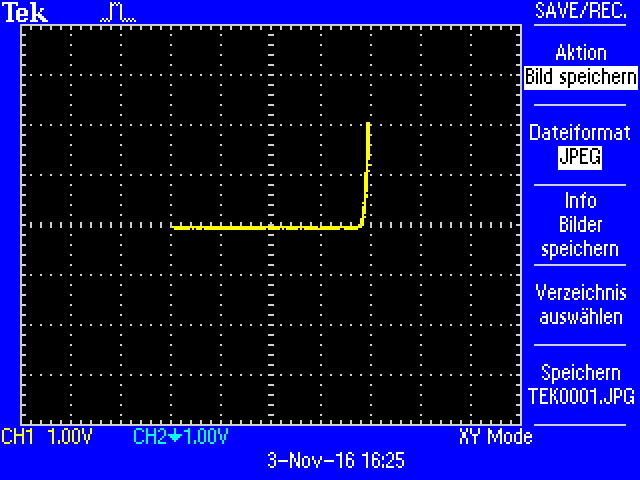
\includegraphics[scale=1]{Daten/TEK0001.JPG}
           \captionof{figure}[DurchlassGerSil]{Kennlinie der roten LED} 
         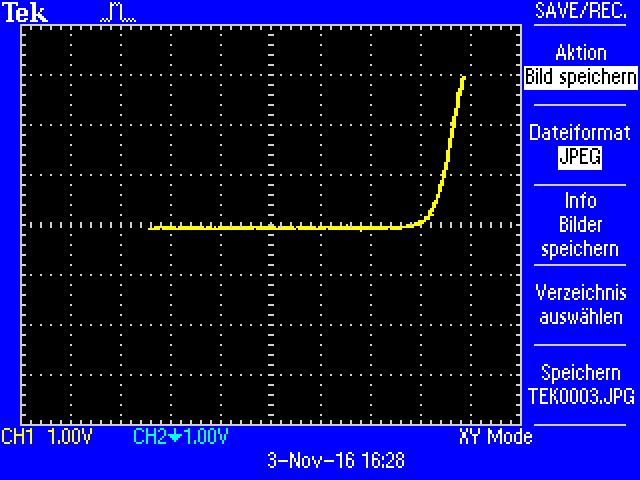
\includegraphics[scale=1]{Daten/TEK0003.JPG}
           \captionof{figure}[DurchlassGerSil]{Kennlinie der blauen LED} 
           \end{center}
        
       Die Schwellspannungen sind aus den Diagrammen abzulesen und sind:
       \begin{center}
       \begin{tabular}{c|c}
       &Schwellspannung\\ \hline
       Rot & $1,8 V$ \\
       Blau & $2,7 V$
       \end{tabular}
       \end{center}
       Damit lässt sich die Wellenlänge des Lichtes berechnen, das von der LED abgestrahlt wird.
       \begin{align*}
       		\lambda_{rot} & = \frac{h \cdot c}{e \cdot U_{rot}} \\
            & = \frac{6,626 \cdot 10^{-34} Js \cdot 0,3 \cdot 10^9 \frac{m}{s}}{1,6 \cdot 10^{-19} C \cdot 1,8 V} = 690,2 nm
       \end{align*} 
       \begin{align*}
       		\lambda_{blau} & = \frac{h \cdot c}{e \cdot U_{blau}} \\
            & = \frac{6,626 \cdot 10^{-34} Js \cdot 0,3 \cdot 10^9 \frac{m}{s}}{1,6 \cdot 10^{-19} C \cdot 2,7 V} = 460,1 nm
       \end{align*}
       
       Die errechneten Wellenlängen passen sehr gut zum Licht, dass von den LEDs abgestrahlt wird, wenn man für blaues Licht eine Wellenlänge von $420nm$ bis $490nm$ und $650nm$ bis $750nm$ für rotes Licht annimmt. \footnote{https://de.wikipedia.org/wiki/Licht}
	\pagebreak


	\chapter{Fehlerrechnung}
	Um das Ventilvolumen in die Formel einzubringen, wird $\gamma$ in Abhängigkeit der Länge $l$, statt der Fläche $A$ und dem Volumen $V$ geschrieben.
      \begin{align*}
     		\gamma = \frac{16 \pi \cdot m \cdot l \cdot f_0^2}{d^2 \cdot p_0}
      \end{align*}
      \begin{align*}
     		\Delta\gamma_{\text{Luft}} &= 
            \left| \frac{16\pi l f_0^2}{d^2 p_0}\right| \Delta m + 
            \left| \frac{16\pi m f_0^2}{d^2 p_0}\right| \Delta l + 
            \left| \frac{32\pi m l f_0}{d^2 p_0}\right| \Delta f_0 + 
            \left| -\frac{32 \pi m l f_0^2}{d^3 p_0}\right| \Delta d \\&+ 
            \left| -\frac{16 \pi m l f_0^2}{d^2 p_0^2}\right| \Delta p_0 \\&=
            \left| \frac{16\pi (0,45m + 0,001m) (13,4Hz)^2}{(0,016m)^2 (103100Pa)}\right| (0,0000001kg)\\ &+ 
            \left| \frac{16\pi (0,0088781kg) (13,4Hz)^2}{(0,016m)^2 (103100Pa)}\right| (0,001m) \\ &+ 
            \left| \frac{32\pi (0,0088781kg) (0,45m + 0,001m) (13,4Hz)}{(0,016m)^2 (103100Pa)}\right| (0,2Hz) \\ &+ 
            \left| -\frac{32 \pi (0,0088781kg) (0,45m + 0,001m) (13,4Hz)^2}{(0,016m)^3 (103100Pa)}\right| (0,00001m)\\&+ 
            \left| -\frac{16 \pi (0,0088781kg) (0,45m + 0,001m) (13,4Hz)^2}{(0,016m)^2 (103100Pa)^2}\right| (100Pa) \\ &= 0,048
      \end{align*} \\
      
      Analog für die weiteren Fehler
      \begin{center}
      \begin{tabular}{c|c}
$l ~[\text{m}]$ & $\Delta\gamma ~[1]$    \\ \hline
0,45         & 0,048 \\
0,40          & 0,045\\
0,35         & 0,045 \\
0,30          & 0,042 \\
0,25         & 0,039 \\
0,20          & 0,037 \\
0,15         & 0,036 \\
0,10          & 0,035	
		\end{tabular}
	\end{center}
      
\captionof{table}[]{Fehler für die Messung mit Luft als Kolbenfüllung.}
\begin{center}
      \begin{tabular}{c|c}
$l ~[\text{m}]$ & $\Delta\gamma ~[1]$    \\ \hline
0,45 & 0,048 \\
0,40  & 0,045 \\
0,35 & 0,042 \\
0,30  & 0,040 \\
0,25 & 0,038 \\
0,20  & 0,036 \\
0,15 & 0,035 \\
0,10  & 0,034
		\end{tabular}
	\end{center}
      
\captionof{table}[]{Fehler für die Messung mit Kohlenstoffdioxid als Kolbenfüllung.}

\begin{center}
      \begin{tabular}{c|c}
$l ~ [\text{m}]$ & $\Delta\gamma ~[1]$    \\ \hline
0,45   & 0,053 \\
0,40    & 0,050 \\
0,35   & 0,048 \\
0,30    & 0,045 \\
0,24   & 0,042 \\
0,19   & 0,038 \\
0,14   & 0,047 \\
0,095  & 0,038 
		\end{tabular}
	\end{center}
      
\captionof{table}[]{Fehler für die Messung mit Argon als Kolbenfüllung.}
\ \\
Es soll nur ein Wert für den Fehler angegeben werden. Anstatt wie bei den Messwerten zu mitteln, wird hier jedoch der größte Fehler angenommen, damit der Fehlerwert nicht zu gering ausfällt.

\begin{align*}
 	\Delta \gamma_{\text{Luft}} & = 0,048\\
    \Delta \gamma_{\text{CO}_2} & = 0,048\\
    \Delta \gamma_{\text{Argon}}& = 0,053
\end{align*}

     	\section{Mögliche Abweichungen}
        	Im Versuch wird angenommen, dass die Erregerfrequenz beim Maximum der Schwingung der Eigenfrequenz des ungedämpften Systems entspricht. Durch Dämpfung fällt die Frequenz jedoch geringer aus, was sich durch den Zusammenhang $\gamma \propto f^2$ stark auf das Ergebnis auswirkt. Der Wert für den gemessenen Adiabatenexponent liegt also unter dem tatsächlichen. Außerdem wird nicht mit einem isolierten System gemessen, sodass der Vorgang nicht vollständig adiabatisch verläuft. Reibung verursacht ebenfalls einen Fehler.
	\pagebreak
		
        
	\chapter{Zusammenfassung}
    
    
    Es wurden der Adiabatenexponenten der Gase Argon, CO$_2$ und Luft (N$_2$) folgende Werte ermittelt: 
    \begin{center}
    
    \begin{tabular}{c|c}
    	Medium & $\gamma ~ [1]$\\ \hline
        Luft & $1,37 \pm 0,048$\\
        CO$_2$ & $1,31 \pm 0,048$\\
        Argon& $1,62 \pm 0,053$
    \end{tabular}
    \captionof{table}[]{Messergebnisse}
    \end{center}
    Fehler erhielt man durch Ungenauigkeiten beim Ablesen der Länge zur Bestimmung der Volumina des Gases. Die Ungenauigkeit beim Ablesen der maximalen Amplitude bei der Resonazfrequenz und die begrenzte Anzeigekapazität des Frequenzgenerators ist auch mit einem gewissen Fehler verbunden.\\
	
	
	\printbibliography
    \pagebreak
    \chapter{Anhang}
    \begin{center}
    		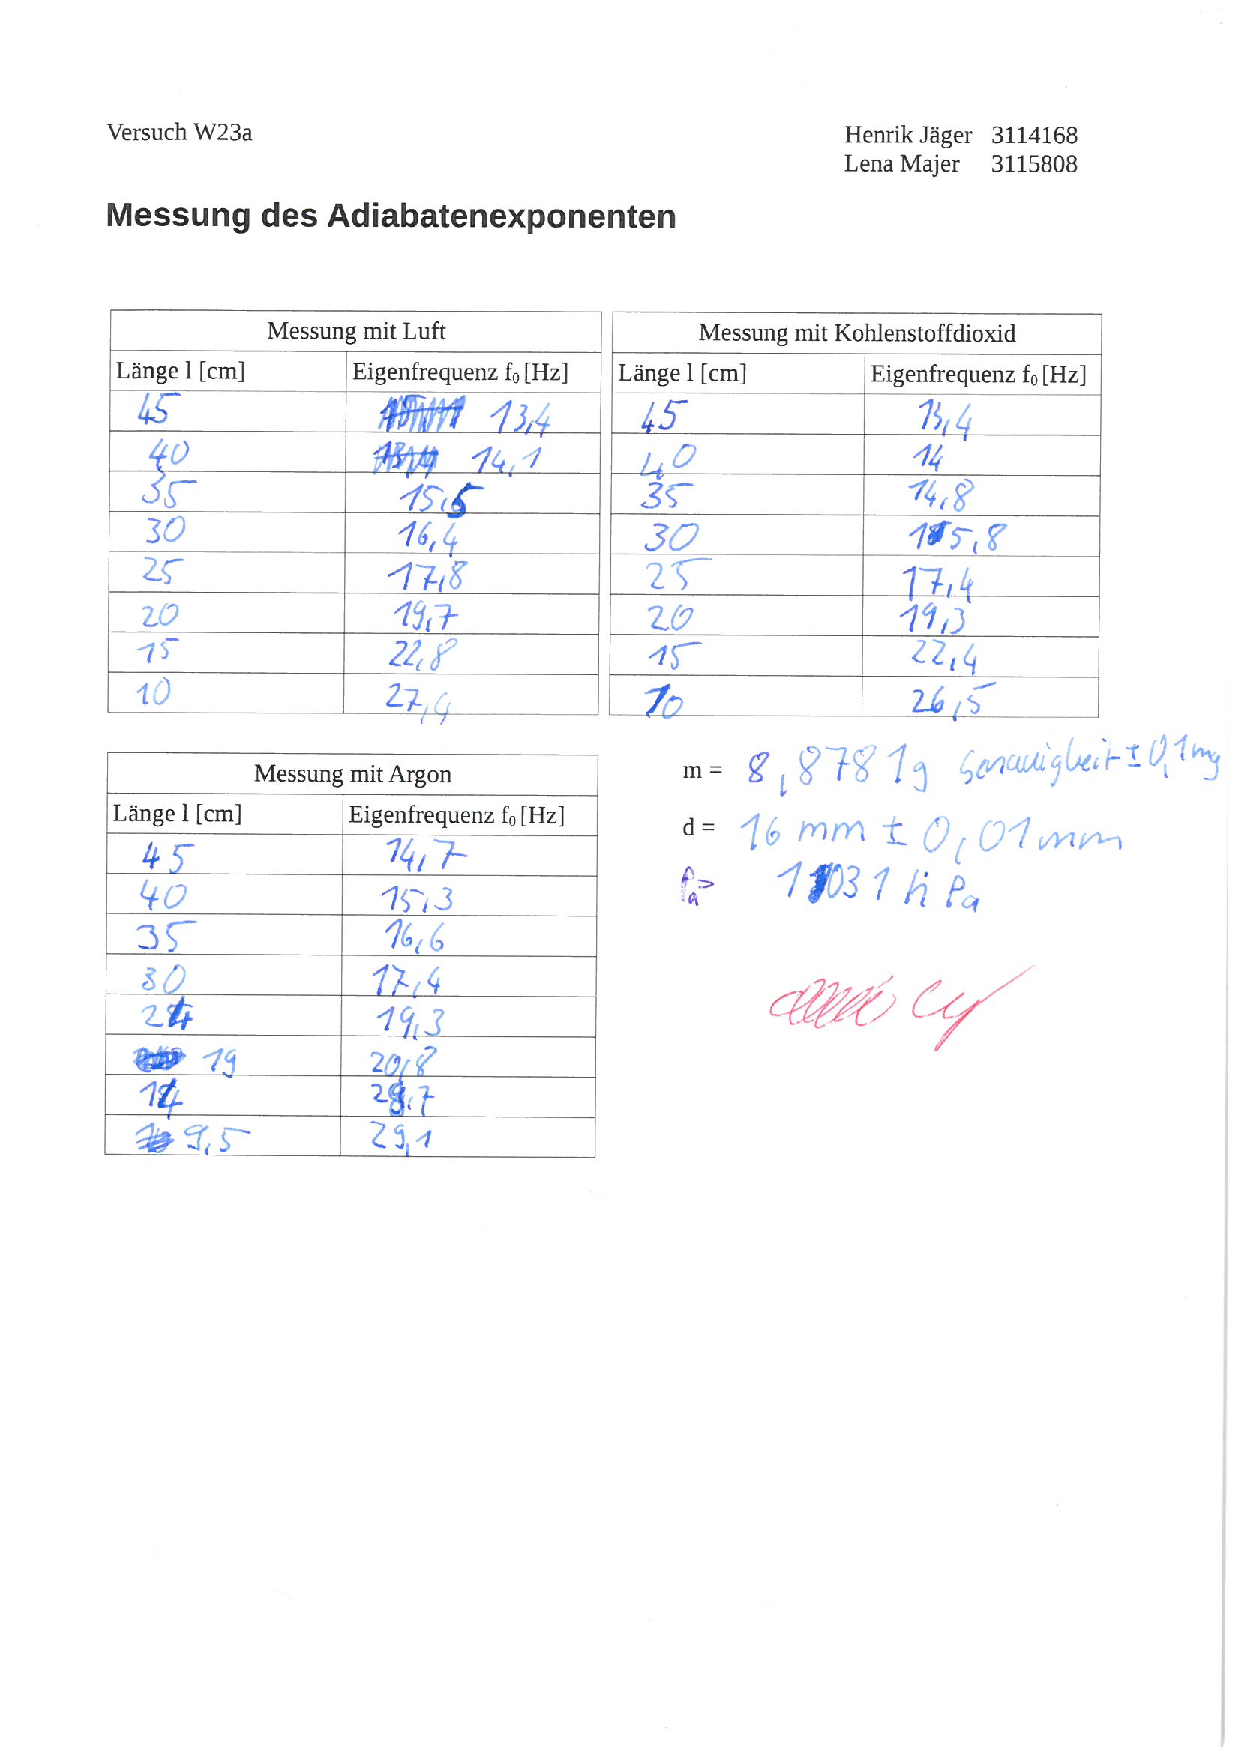
\includegraphics[scale=0.65]{Daten/protokoll.pdf}
    	\end{center}
    	\captionof{figure}[Seite 1]{Messprotokoll}
	\pagebreak








\end{document}
